%General help: texdoc 
%e.g. texdoc amsmath
\documentclass{article}
\title{First Document}

\usepackage{amsmath}
\usepackage{graphicx}
\usepackage{booktabs} %for \toprule (mid,bottom)
\usepackage{siunitx} % formats the units and values.
%Setup siunitx:
\sisetup{
	round-mode=places, %rounds numbers
	round-precision=2, %to 2 places
}
\usepackage{pgfplotstable} %generates table from .csv
%\usepackage[backend=bibtex,style=verbose-trad2]{biblatex}
%\bibliography{my}


%about circuit
\usepackage{circuitikz}


%%plot image.
\usepackage{tikz}
\usepackage{pgfplots}
\pgfplotsset{compat=newest}
%\pgfplotsset{compat=1.9}
\usepgfplotslibrary{units}


%Unused.
%\usepackage{listings}
%\renewcommand{\lstlistingname}{Algorithm}
%\renewcommand{\lstlistlistingname}{List of \lstlistingname s}


%about source code highlighting
%using minted to highlight source code
\usepackage{minted}
\renewcommand\listingscaption{Algorithm}
\renewcommand\listoflistingscaption{List of \listingscaption s}

\newmintedfile[cppfile]{cpp}{frame=lines,linenos}
%\usemintedstyle{colorful}




\date{2016-4-7}

\author{EricLin}


\begin{document}
\pagenumbering{gobble}
\maketitle

\begin{minted}{c}
	int main(){
		printf("hello,    world");
		return 0;
	}
\end{minted}


\inputminted{cpp}{main.cpp}


New method:
\begin{listing}[H]
	\cppfile{main.cpp}
	\caption{below the code}
	\label{lst:previous-main}
\end{listing}

I'm refering to the Listing \ref{lst:main}, end.




\newpage
\begin{figure}[h!]
	\begin{center}
		\begin{circuitikz}
			\draw(0,0)
			to [V,v=$U_q$] (0,2)
			to [short] (2,2)
			to [R=$R_1$](2,0)
			to [short](0,0);
		\end{circuitikz}
	\end{center}
\end{figure}
\begin{figure}[h!]
	%\begin{center}
	\caption{My autogenerated plot.}
	\begin{tikzpicture}
		\draw[red,dashed](0,0) rectangle(4,4) node [black,below]{Start};
		\draw[thick](2,2) 
		to [out=0,in=0](8,2)
		to [out=0,in=0](2,-4);
		%node is text-node
		\draw[fill](8-2,2-0.1) rectangle (8+2,2+0.1) node[black,right]{Obstacle};
		\draw[red,fill](2,-4) circle [radius=0.2] node[black,below=4]{Point of interest};
		\begin{axis}[
				width=\linewidth,
				grid=major,
				grid style={dashed,gray!30},
				xlabel=X axis $U$,
				ylabel=Y asix $I$,
				x unit=\si{\volt},
				y unit=\si{\ampere},
				legend style={at={(0.8,0.8)},anchor=north},
				x tick label style={rotate=90}
			]
			\addplot
			table[x=A, y=V, col sep=comma]{table.csv};
			\legend{$f(x)=x^2+3x+5$}
		\end{axis}
	\end{tikzpicture}
	%\end{center}
\end{figure}
\begin{table}[h!]
	\begin{center}
		\caption{Autogenerated table from .csv file.}
		\label{g1}
		\pgfplotstabletypeset[
			multicolumn names,
			col sep=comma,
			display columns/0/.style={%change the column's name.
				column name=$Value 1$,
				column type={S},string type
			},
			display columns/1/.style={
				column name=$Value 2$,
				column type={S},string type
			},
			display columns/2/.style={
				column name=$Value 3$,
				column type={S},string type
			},
			every head row/.style={
				before row={\toprule},
				after row={
					\si{\ampere}&\si{\volt}&\si{\tesla}\\
				\midrule}
			},
			every last row/.style={
				after row=\bottomrule
			},
		]{table.csv}
	\end{center}
\end{table}
$fuck you$ hello<F5>
\newpage
this is footnote\footnote{\label{foo1}Hello footnote}.
this is footnote2\footnote{\label{foo2}Hello footnote}.
i'm referring to previous footnote\ref{foo2}.
i'm referring to first footnote\ref{foo1}.
\begin{table}[h!]
	\centering
	\caption{My Table}
	\label{table:abc}
	\begin{tabular}{c|||c||r|c|c}
		1&2&3\\
		\hline
		\hline
		\hline
		a&b&c\\
	\end{tabular}
\end{table}

\begin{table}[h!]
	\centering
	\caption{mytable2}
	\begin{tabular}{ccc}
		\toprule
		Some &actual&content\\
		\midrule
		prettifies &the& table\\
		as &wel &as\\
		using &the& booktabs package\\
		\bottomrule
	\end{tabular}
\end{table}


\newpage
\tableofcontents

\newpage

\pagenumbering{arabic}

\begin{figure}
	\caption{dummy figure}
\end{figure}



\begin{figure}[h!]
	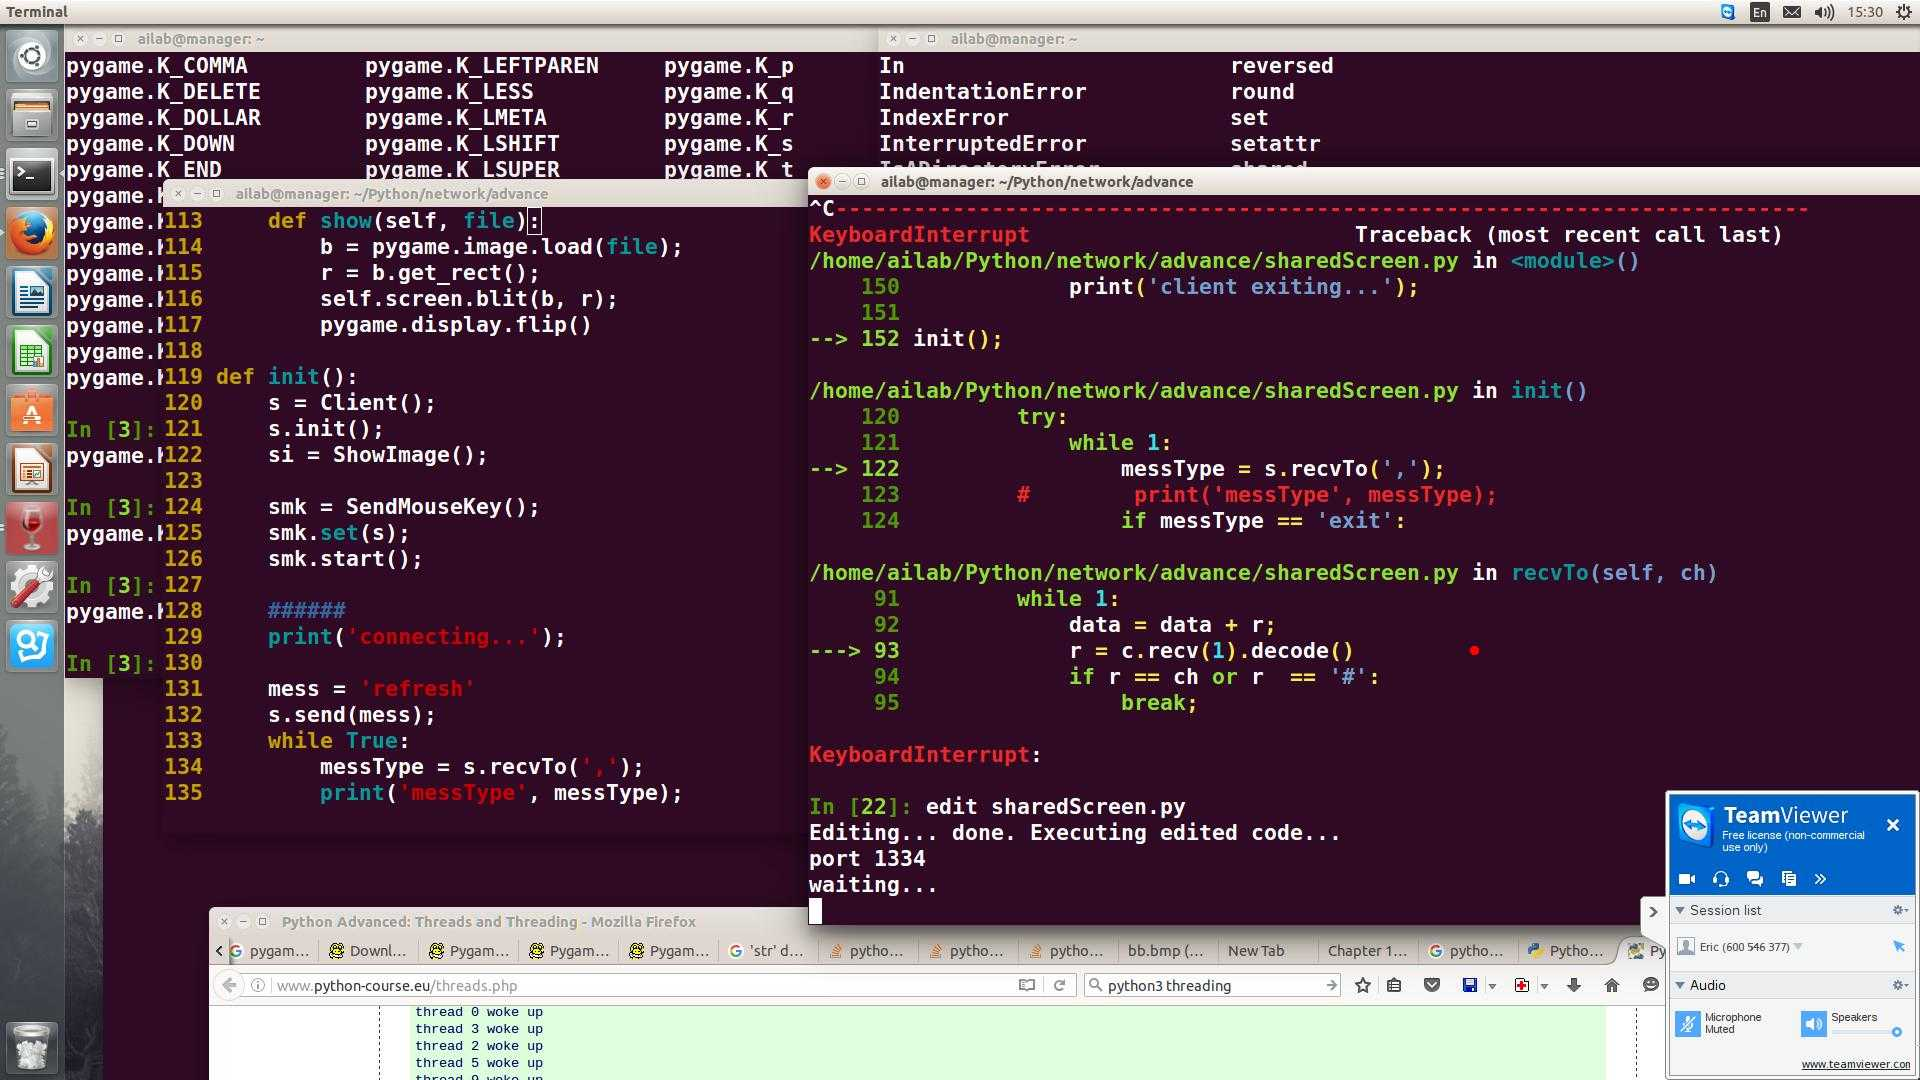
\includegraphics[width=\linewidth]{tmp.jpg}
	\caption{A tmp jpg what?}
	\label{fig:tmpa}
\end{figure}
\begin{figure}
	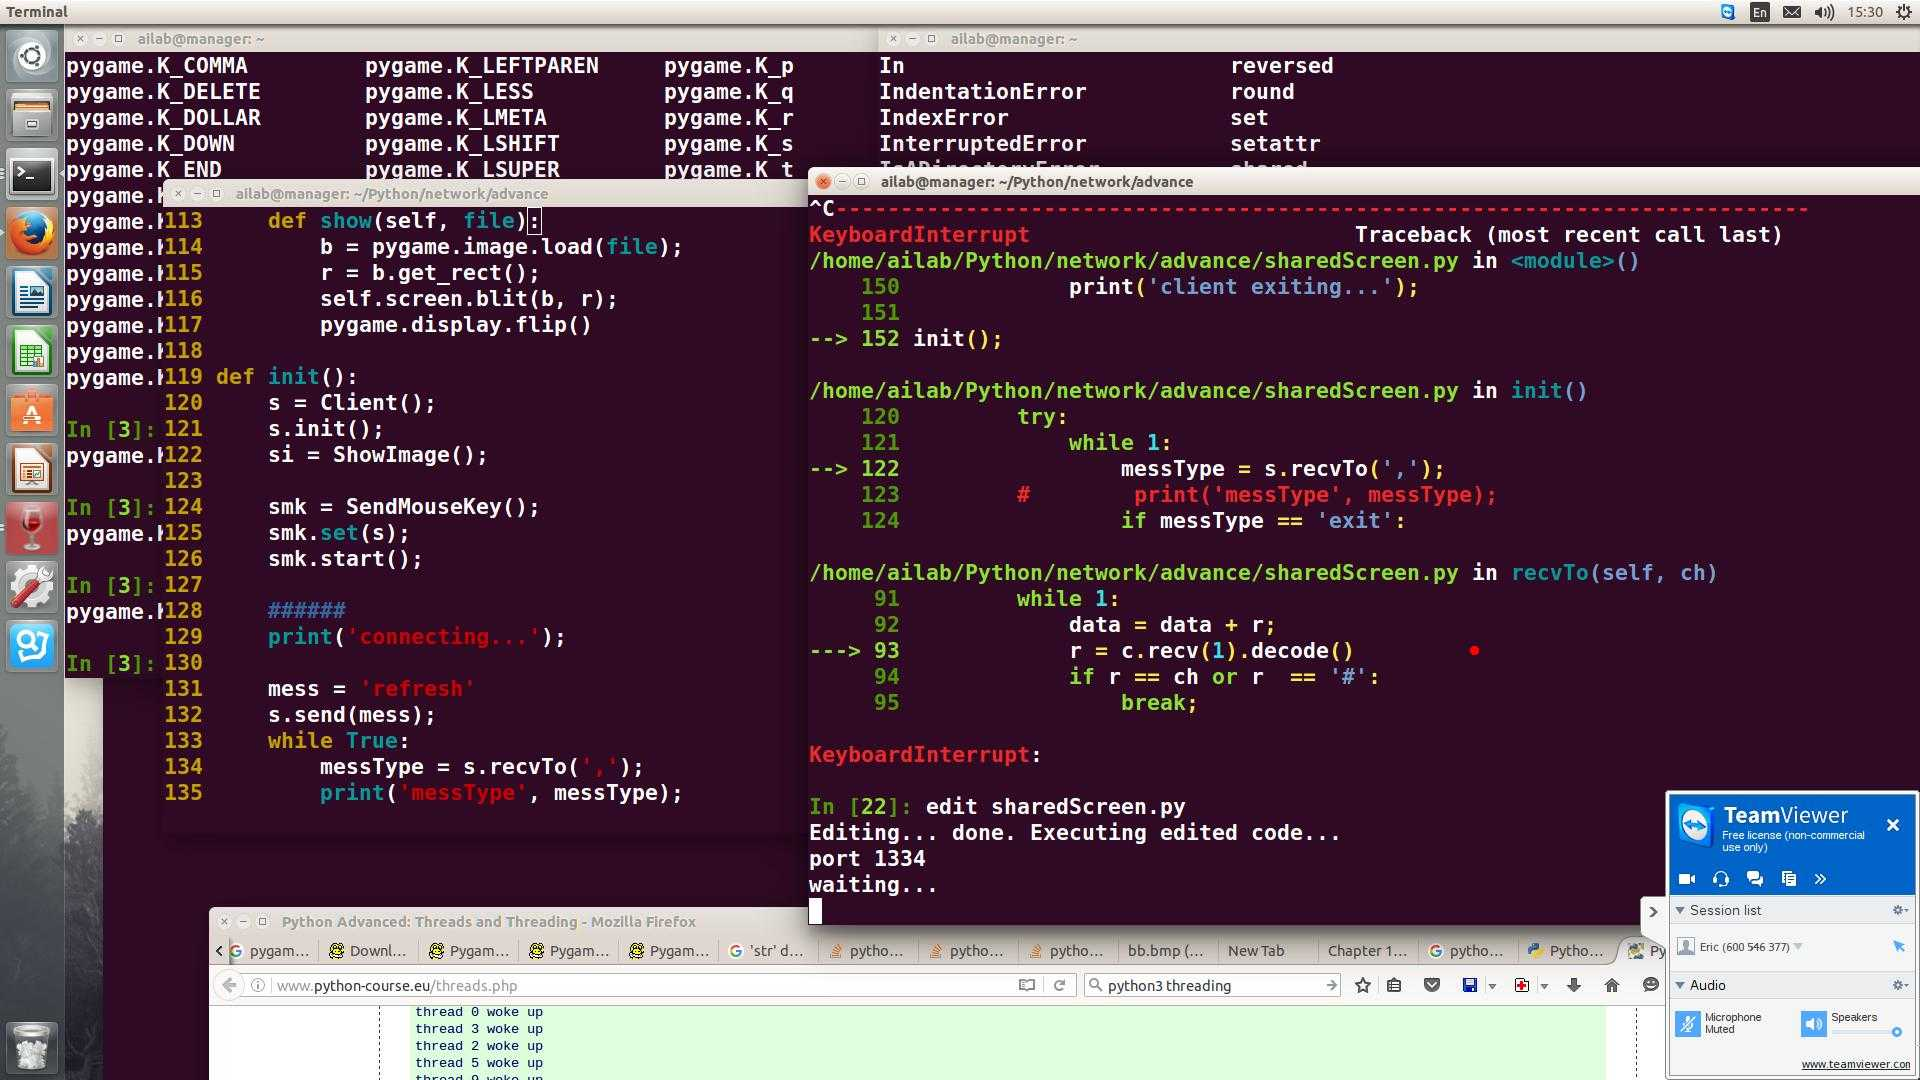
\includegraphics[width=\linewidth]{tmp.jpg}
	\caption{A tmp jpg}
	\label{fig:tmp}
\end{figure}
Figure \ref{fig:tmp} show a tmp jpg.


%some comment
Figure \ref{fig:tmpa} show a tmp jpg.

\begin{equation*}
	f(x)=x^2
	y=ax^2+bx+c
\end{equation*}
\begin{equation*}
	1+2 =3
\end{equation*}
\begin{align}
	1+2&=3\\
	1&=3-2
\end{align}
\begin{align}
	f(x)=x^2\\
	g(x)=\frac{1}{x}\\
	F(x)=\int^a_b    \frac{1}{3}x^3\\
	IntF(x)=\int_a^b    \frac{1}{3}x^3\\
	ClosedIntgral(x)=\oint_D F ds\\
	c(x)=\frac{f(x)}{\frac{4}{3}}\\
	\left(d(x)=\frac{1}{\sqrt{x}}\right)\\
	\left[
		\begin{matrix}
			1&0&3\\
			1&0&3\\
			2&4
		\end{matrix}
	\right]\\
	\lambda^2
	\alpha
	\beta
	\theta
\end{align}

adfadfadf\\zverqwerqewraf

The formula is $f(x)=x^2$, for example.
\newpage


\newpage
\section{section1}
Hello World!


adf
adf

afd
a
f
\subsection{section2}
sub section
\paragraph{new paragraph}
some text.
next line

\newpage
new hello
New method:
\begin{listing}[h!]
	\cppfile{main.cpp}
	\caption{below the code}
	\label{lst:main}
\end{listing}
\newpage
hello
\begin{table}
	\caption{Dummy table}
\end{table}
%rnadom citation \autocite[5]{dummybook:1}
rnadom citation \cite{dummybook:1} bibtex

\begin{table}
	\caption{Dummy2 table}
\end{table}
\newpage
\begin{appendix}
	\listoffigures
	\listoftables
	\listoflistings
\end{appendix}

\newpage
biblatex references:
%\printbibliography

bibtex references:
\bibliography{my}
\bibliographystyle{ieeetr}



\end{document}
